%----------------------------------------------------------------------------------------
%	PACKAGES AND THEMES
%----------------------------------------------------------------------------------------
\documentclass[a4paper,12pt]{article}
\usepackage[english]{babel}
\usepackage[utf8]{inputenc}

\usepackage{listings}
\usepackage{color}
\renewcommand\lstlistingname{Quelltext} % Change language of section name
\lstset{ % General setup for the package
    language=Perl,
    basicstyle=\small\sffamily,
    numbers=left,
     numberstyle=\tiny,
    frame=tb,
    tabsize=4,
    columns=fixed,
    showstringspaces=false,
    showtabs=false,
    keepspaces,
    commentstyle=\color{red},
    keywordstyle=\color{blue}
}

\usepackage{graphicx}

%
% For alternative styles, see the biblatex manual:
% http://mirrors.ctan.org/macros/latex/contrib/biblatex/doc/biblatex.pdf
%
% The 'verbose' family of styles produces full citations in footnotes, 
% with and a variety of options for ibidem abbreviations.
%
\usepackage{csquotes}
\usepackage[style=verbose-ibid,backend=bibtex]{biblatex}
\bibliography{sample}

\usepackage{lipsum} % for dummy text

%----------------------------------------------------------------------------------------
%	Main Page PAGE
%----------------------------------------------------------------------------------------

\title{Text analysis of Trump’s tweets confirms he writes only the
(angrier) Android half}
\author{David Robinson}
\date{August 2016}
\begin{document}
\maketitle
%------------------------------------------------

I don’t normally post about politics (I’m not particularly savvy about polling, which is where
data science has had the largest impact on politics). But this weekend I saw a hypothesis about
Donald Trump’s twitter account that simply begged to be investigated with data; see Figure 1.
When Trump wishes the Olympic team good luck, he’s tweeting from his iPhone. When he’s
insulting a rival, he’s usually tweeting from an Android. Is this an artifact showing which tweets
are Trump’s own and which are by some handler?
Others have explored Trump’s timeline and noticed this tends to hold up- and Trump himself
does indeed tweet from a Samsung Galaxy. But how could we examine it quantitatively? I’ve been
writing about text mining and sentiment analysis [1] recently, particularly during my development
of the tidytext R package with Julia Silge, and this is a great opportunity to apply it again.
My analysis, shown below, concludes that the Android and iPhone tweets are clearly from
different people, posting during different times of day and using hashtags, links, and retweets
in distinct ways. What’s more, we can see that the Android tweets are angrier and more
negative, while the iPhone tweets tend to be benign announcements and pictures. Overall I’d agree
with @tvaziri’s analysis: this lets us tell the difference between the campaign’s tweets (iPhone) and
Trump’s own (Android).
%------------------------------------------------

\section{The Dataset}
First we’ll retrieve the content of Donald Trump’s timeline using the userTimeline function in the
twitteR package:1
%------------------------------------------------

%------------------------------------------------

\begin{lstlisting}
library(dplyr)
library(purrr)
library(twitteR)
\end{lstlisting}

%------------------------------------------------

 %Adding picture
  \begin{figure}[h!]
  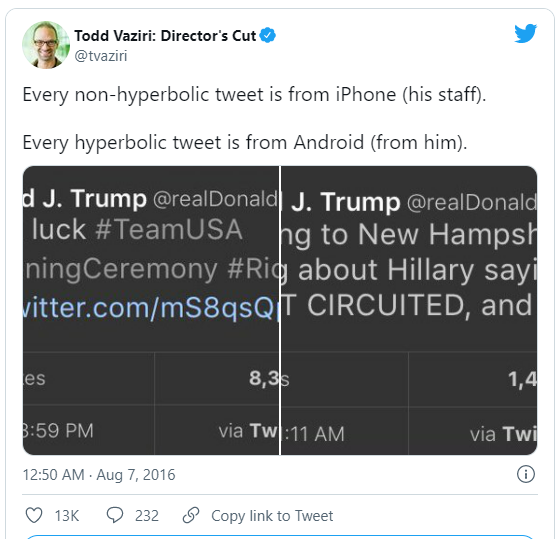
\includegraphics[width=\linewidth]{Tweet.png}
  \caption{Sanjay K V.}
  \label{fig:Tweet by Todd Vaziri}
\end{figure}
%------------------------------------------------



\begin{lstlisting}
# You'd need to set global options with an authenticated app
setup_twitter_oauth(getOption("twitter_consumer_key"),
                    getOption("twitter_consumer_secret"),
                    getOption("twitter_access_token"),
                    getOption("twitter_access_token_secret"))
# We can request only 3200 tweets at a time; it will return fewer
# depending on the API
trump_tweets <- userTimeline("realDonaldTrump", n = 3200)
trump_tweets_df <- tbl_df(map_df(trump_tweets, as.data.frame))
\end{lstlisting}

%------------------------------------------------

%second code
\begin{lstlisting}
# if you want to follow along without setting up Twitter authentication,
# just use my dataset:
load(url("http://varianceexplained.org/files/trump_tweets_df.rda"))
\end{lstlisting}
\printbibliography
%------------------------------------------------

%third code
\begin{lstlisting}
library(tidyr)

tweets <- trump_tweets_df %>%
  select(id, statusSource, text, created) %>%
  extract(statusSource, "source", "Twitter for (.*?)<") %>%
  filter(source %in% c("iPhone", "Android"))
  \end{lstlisting}
%------------------------------------------------

  
  %Adding picture
  \begin{figure}[h!]
  \includegraphics[width=\linewidth]{Chunk.png}
  \caption{Sanjay K V.}
  \label{fig:Tweet by Todd Vaziri}
\end{figure}
Overall, this includes 628 tweets from iPhone, and 762 tweets from Android.

One consideration is what time of day the tweets occur, which we’d expect to be a “signature” of their user. Here we can certainly spot a difference:


%------------------------------------------------

%third code
\begin{lstlisting}
library(lubridate)
library(scales)

tweets %>%
  count(source, hour = hour(with_tz(created, "EST"))) %>%
  mutate(percent = n / sum(n)) %>%
  ggplot(aes(hour, percent, color = source)) +
  geom_line() +
  scale_y_continuous(labels = percent_format()) +
  labs(x = "Hour of day (EST)",
       y = "% of tweets",
       color = "")
  \end{lstlisting}
  %------------------------------------------------

  
  Trump on the Android does a lot more tweeting in the morning, while the campaign posts from the iPhone more in the afternoon and early evening.

Another place we can spot a difference is in Trump’s anachronistic behavior of “manually retweeting” people by copy-pasting their tweets, then surrounding them with quotation marks:


%----------------------------------------------------------------------------------------
%  PAGE 4
%----------------------------------------------------------------------------------------
\section{Comparison of words}
Now that we’re sure there’s a difference between these two accounts, what can we say about the difference in the content? We’ll use the tidytext package that Julia Silge and I developed.

We start by dividing into individual words using the unnest_tokens function (see this vignette for more), and removing some common “stopwords”2:

%third code
\begin{lstlisting}
library(tidytext)

reg <- "([^A-Za-z\\d#@']|'(?![A-Za-z\\d#@]))"
tweet_words <- tweets %>%
  filter(!str_detect(text, '^"')) %>%
  mutate(text = str_replace_all(text, "https://t.co/[A-Za-z\\d]+|&amp;", "")) %>%
  unnest_tokens(word, text, token = "regex", pattern = reg) %>%
  filter(!word %in% stop_words$word,
         str_detect(word, "[a-z]"))

tweet_words
  \end{lstlisting}
 %------------------------------------------------
  
%Fourth code
\begin{lstlisting}
## # A tibble: 8,753 x 4
##                    id source             created                   word
##                 <chr>  <chr>              <time>                  <chr>
## 1  676494179216805888 iPhone 2015-12-14 20:09:15                 record
## 2  676494179216805888 iPhone 2015-12-14 20:09:15                 health
## 3  676494179216805888 iPhone 2015-12-14 20:09:15 #makeamericagreatagain
## 4  676494179216805888 iPhone 2015-12-14 20:09:15             #trump2016
## 5  676509769562251264 iPhone 2015-12-14 21:11:12               accolade
## 6  676509769562251264 iPhone 2015-12-14 21:11:12             @trumpgolf
## 7  676509769562251264 iPhone 2015-12-14 21:11:12                 highly
## 8  676509769562251264 iPhone 2015-12-14 21:11:12              respected
## 9  676509769562251264 iPhone 2015-12-14 21:11:12                   golf
## 10 676509769562251264 iPhone 2015-12-14 21:11:12                odyssey
## # ... with 8,743 more rows
  \end{lstlisting}  
  %------------------------------------------------
These should look familiar for anyone who has seen the feed. Now let’s consider which words are most common from the Android relative to the iPhone, and vice versa. We’ll use the simple measure of log odds ratio, calculated for each word as:3


# in Android+1
total Android+1
# in iPhone+1
total iPhone+1

  
  %Adding picture
  \begin{figure}
  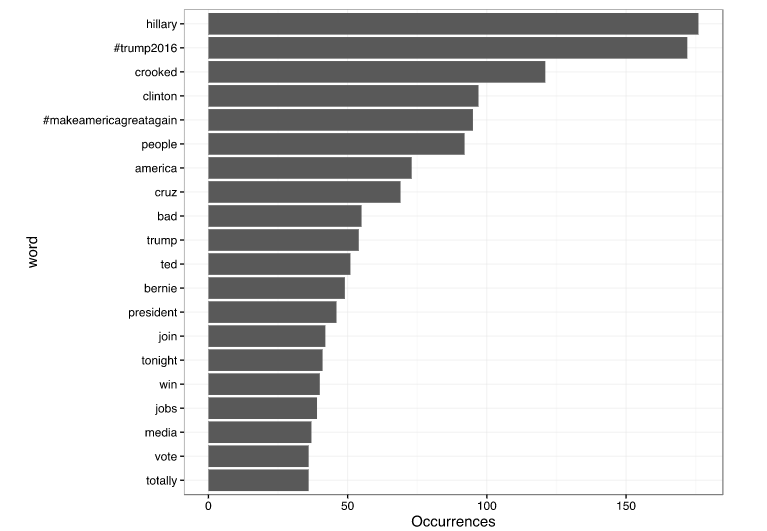
\includegraphics[width=\linewidth]{bar-chart.png}
  \caption{Sanjay K V.}
  \label{fig:Tweet words plot}
\end{figure}

To measure the sentiment of the Android and iPhone tweets, we can count the number of words in each category:

 %------------------------------------------------
  
%Fifth code
\begin{lstlisting}
sources <- tweet_words %>%
  group_by(source) %>%
  mutate(total_words = n()) %>%
  ungroup() %>%
  distinct(id, source, total_words)

by_source_sentiment <- tweet_words %>%
  inner_join(nrc, by = "word") %>%
  count(sentiment, id) %>%
  ungroup() %>%
  complete(sentiment, id, fill = list(n = 0)) %>%
  inner_join(sources) %>%
  group_by(source, sentiment, total_words) %>%
  summarize(words = sum(n)) %>%
  ungroup()

head(by_source_sentiment)
  \end{lstlisting}  
    This gives counts as in Table 1
  %------------------------------------------------

  \begin{table}[h!]
  \begin{center}
    \caption{Emotion Counts.}
    \label{tab:table1}
    \begin{tabular}{o\l|c|r|u} % <-- Alignments: 1st column left, 2nd middle and 3rd right, with vertical lines in between
      \textbf{ } & \textbf{Source} & \textbf{sentiment} & \textbf{total words} & \textbf{words}\\
      
      \hline
      1 & Android & anger & 4901 & 321 \\
      2 & Android & anticipation & 4901 & 256\\
      3 & Android & disgust & 4901 & 207\\
      3 & Android & fear & 4901 & 268\\
      3 & Android & joy & 4901 & 199\\
      3 & Android & negative & 4901 & 560\\
    \end{tabular}
  \end{center}
\end{table}
  
  %----------------------------------------------------------------------------------------
%  PAGE 6
%----------------------------------------------------------------------------------------
\section{Reference}
\end{document}